\section{Results of the Runtime Verified AV System}

This research provides a solution for two aspects of \acf{AV} systems: predicting accurately with perturbations to the system's inputs and safely dealing with misclassifications by the system.
The issue of input perturbations was addressed using a \acf{MNN} of different convolutional \acfp{SNN}, each \ac{SNN} working in tandem to predict more accurately.
Misclassification by the system's controller was addressed by implementing sensor fusion between cameras and \ac{LiDAR}.
This was done using a run-time enforcer that enforced a safety automaton.

\todo{fix results with new graphs}

To test the \ac{MNN}'s ability to deal with perturbations, the input images (taken from the \ac{VOC} 2012 and \ac{GTSRB} datasets) were perturbed by randomly replacing approximately 7\% of the image pixels with randomly coloured pixels.
Table~\ref{tbl:sign-res} shows that without perturbations, the accuracy of the \ac{MNN} was increased from 87.07\% to 93.7\% when using an enforced policy.
Table~\ref{tbl:sign-respert} shows that the accuracy of the \ac{MNN} hugely decreases when perturbations are present, from 87.07\% to 41.6\%.
However, with sensor fusion and a relative safety policy, the accuracy is increased to 90.48\%.
 
\begin{table}[h]
	\centering
	\resizebox{\textwidth}{!}{%
		\begin{tabular}{|p{0.17\linewidth}||p{0.17\linewidth}|p{0.17\linewidth}|p{0.17\linewidth}|p{0.17\linewidth}|}
			\hline
			Object classified & No. of misclassifications (\%) & Caught misclassifications (\%) & False negatives (\%) & Uncaught misclassifications (\%) \\ \hline
			Person & 17.01 & 17.01 & 0.00 & 0.00 \\ \hline
			Vehicle & 15.85 & 15.85 & 0.00 & 0.00 \\ \hline
			Sign & 54.46 & 54.46 & 4.84 & 4.84 \\ \hline
			Nothing & 7.83 & 7.83 & 0.00 & 0.00 \\ \hline
			All & 95.16 & 95.16 & 4.84 & 4.84 \\ \hline
		\end{tabular}%
	}
	\caption{Table showing the worst results of the \ac{AV} prediction \ac{SNN} using the original images, trained for 0 epochs}
	\label{tbl:sign-res1}
\end{table}

\begin{table}[h]
	\centering
	\resizebox{\textwidth}{!}{%
		\begin{tabular}{|p{0.17\linewidth}||p{0.17\linewidth}|p{0.17\linewidth}|p{0.17\linewidth}|p{0.17\linewidth}|}
			\hline
			Object classified & No. of misclassifications (\%) & Caught misclassifications (\%) & False negatives (\%) & Uncaught misclassifications (\%) \\ \hline
			Person & 1.00 & 0.21 & 0.53 & 1.32 \\ \hline
			Vehicle & 6.26 & 5.63 & 0.44 & 1.07 \\ \hline
			Sign & 2.62 & 0.44 & 1.02 & 3.20 \\ \hline
			Nothing & 2.50 & 2.27 & 0.12 & 0.35 \\ \hline
			All & 12.38 & 8.55 & 2.11 & 5.93 \\ \hline
		\end{tabular}%
	}
	\caption{Table showing results of the \ac{AV} prediction \ac{SNN} using the original images, trained for 10000 epochs}
	\label{tbl:sign-res10000}
\end{table}

\begin{table}[h]
	\centering
	\resizebox{\textwidth}{!}{%
		\begin{tabular}{|p{0.17\linewidth}||p{0.17\linewidth}|p{0.17\linewidth}|p{0.17\linewidth}|p{0.17\linewidth}|}
			\hline
			Object classified & No. of misclassifications (\%) & Caught misclassifications (\%) & False negatives (\%) & Uncaught misclassifications (\%) \\ \hline
			Person & 1.11 & 0.70 & 0.65 & 1.07 \\ \hline
			Vehicle & 3.92 & 3.34 & 0.65 & 1.23 \\ \hline
			Sign & 2.64 & 0.60 & 0.51 & 2.55 \\ \hline
			Nothing & 2.92 & 2.69 & 0.23 & 0.46 \\ \hline
			All & 10.59 & 7.32 & 2.04 & 5.31 \\ \hline
		\end{tabular}%
	}
	\caption{Table showing the best results of the \ac{AV} prediction \ac{SNN} using the original images, trained for 6000 epochs}
	\label{tbl:sign-resbest}
\end{table}

\begin{table}[h]
	\centering
	\resizebox{\textwidth}{!}{%
		\begin{tabular}{|p{0.17\linewidth}||p{0.17\linewidth}|p{0.17\linewidth}|p{0.17\linewidth}|p{0.17\linewidth}|}
			\hline
			Object classified & No. of misclassifications (\%) & Caught misclassifications (\%) & False negatives (\%) & Uncaught misclassifications (\%) \\ \hline
			Person & 17.01 & 17.01 & 0.00 & 0.00 \\ \hline
			Vehicle & 15.85 & 15.85 & 0.00 & 0.00 \\ \hline
			Sign & 54.46 & 54.46 & 4.84 & 4.84 \\ \hline
			Nothing & 7.83 & 7.83 & 0.00 & 0.00 \\ \hline
			All & 95.16 & 95.16 & 4.84 & 4.84 \\ \hline
		\end{tabular}%
	}
	\caption{Table showing the worst results of the \ac{AV} prediction \ac{SNN} using perturbed images, trained for 0 epochs}
	\label{tbl:sign-respert1}
\end{table}

\begin{table}[h]
	\centering
	\resizebox{\textwidth}{!}{%
		\begin{tabular}{|p{0.17\linewidth}||p{0.17\linewidth}|p{0.17\linewidth}|p{0.17\linewidth}|p{0.17\linewidth}|}
			\hline
			Object classified & No. of misclassifications (\%) & Caught misclassifications (\%) & False negatives (\%) & Uncaught misclassifications (\%) \\ \hline
			Person & 3.43 & 0.60 & 0.56 & 3.38 \\ \hline
			Vehicle & 10.78 & 8.57 & 0.23 & 2.43 \\ \hline
			Sign & 38.08 & 31.91 & 1.39 & 7.56 \\ \hline
			Nothing & 5.61 & 4.80 & 0.09 & 0.90 \\ \hline
			All & 57.89 & 45.89 & 2.27 & 14.28 \\ \hline
		\end{tabular}%
	}
	\caption{Table showing results of the \ac{AV} prediction \ac{SNN} using perturbed images, trained for 10000 epochs}
	\label{tbl:sign-respert10000}
\end{table}

\begin{table}[h]
	\centering
	\resizebox{\textwidth}{!}{%
		\begin{tabular}{|p{0.17\linewidth}||p{0.17\linewidth}|p{0.17\linewidth}|p{0.17\linewidth}|p{0.17\linewidth}|}
			\hline
			Object classified & No. of misclassifications (\%) & Caught misclassifications (\%) & False negatives (\%) & Uncaught misclassifications (\%) \\ \hline
			Person & 3.22 & 1.02 & 0.79 & 2.99 \\ \hline
			Vehicle & 9.20 & 7.25 & 0.53 & 2.48 \\ \hline
			Sign & 33.30 & 27.65 & 2.71 & 8.37 \\ \hline
			Nothing & 6.81 & 6.12 & 0.09 & 0.79 \\ \hline
			All & 52.54 & 42.04 & 4.13 & 14.62 \\ \hline
		\end{tabular}%
	}
	\caption{Table showing the best results of the \ac{AV} prediction \ac{SNN} using perturbed images, trained for 700 epochs}
	\label{tbl:sign-respertbest}
\end{table}

\begin{figure}[t]
	\centering
	\scalebox{1}{\begin{tikzpicture}
\begin{semilogxaxis}[
xlabel={Number of epochs trained},
ylabel={\% of total classifications},
x=1.1cm,
y=1.0mm, 
legend style={at={(0.55,0.9)},anchor=west}]

\addplot[color=black,mark=x] coordinates {
	(1, 100.000000)
	(10, 100.000000)
	(20, 99.968513)
	(30, 99.438622)
	(40, 98.948822)
	(50, 99.831619)
	(60, 100.000000)
	(70, 99.946243)
	(80, 98.629845)
	(90, 99.235352)
	(100, 73.896217)
	(200, 67.904327)
	(300, 73.114166)
	(400, 71.500191)
	(500, 73.917786)
	(600, 72.264412)
	(700, 71.438644)
	(800, 70.175438)
	(900, 70.787399)
	(1000, 72.854225)
	(2000, 70.439842)
	(3000, 69.480080)
	(4000, 67.477409)
	(5000, 68.717560)
	(6000, 69.121811)
	(7000, 70.645164)
	(8000, 67.972473)
	(9000, 68.772896)
	(10000, 69.063011)
	(20000, 67.405907)
	(30000, 69.780220)
	(40000, 67.787842)
	(50000, 69.032257)
	(60000, 68.315018)
	(70000, 68.693977)
	(80000, 70.194382)
	(90000, 69.604439)
	(100000, 65.025040)
};

\addplot[color=brown,mark=x] coordinates {	
	(1, 0.000000)
	(10, 0.000000)
	(20, 0.031486)
	(30, 0.561380)
	(40, 1.051184)
	(50, 0.168381)
	(60, 0.000000)
	(70, 0.053759)
	(80, 1.370155)
	(90, 0.764649)
	(100, 26.103786)
	(200, 32.095673)
	(300, 26.885832)
	(400, 28.499805)
	(500, 26.082212)
	(600, 27.735594)
	(700, 28.561354)
	(800, 29.824560)
	(900, 29.212601)
	(1000, 27.145777)
	(2000, 29.560154)
	(3000, 30.519920)
	(4000, 32.522587)
	(5000, 31.282434)
	(6000, 30.878185)
	(7000, 29.354836)
	(8000, 32.027523)
	(9000, 31.227106)
	(10000, 30.936995)
	(20000, 32.594090)
	(30000, 30.219782)
	(40000, 32.212166)
	(50000, 30.967743)
	(60000, 31.684982)
	(70000, 31.306025)
	(80000, 29.805618)
	(90000, 30.395559)
	(100000, 34.974957)
};


\legend{Caught misclassifications, Uncaught misclassifications}
\end{semilogxaxis}%
\end{tikzpicture}%}
	\caption{Line graph showing the performance of the system trained over an increasing amount of epochs using unperturbed inputs \label{fig:sign-graph}}
\end{figure}

\begin{figure}[t]
	\centering
	\scalebox{1}{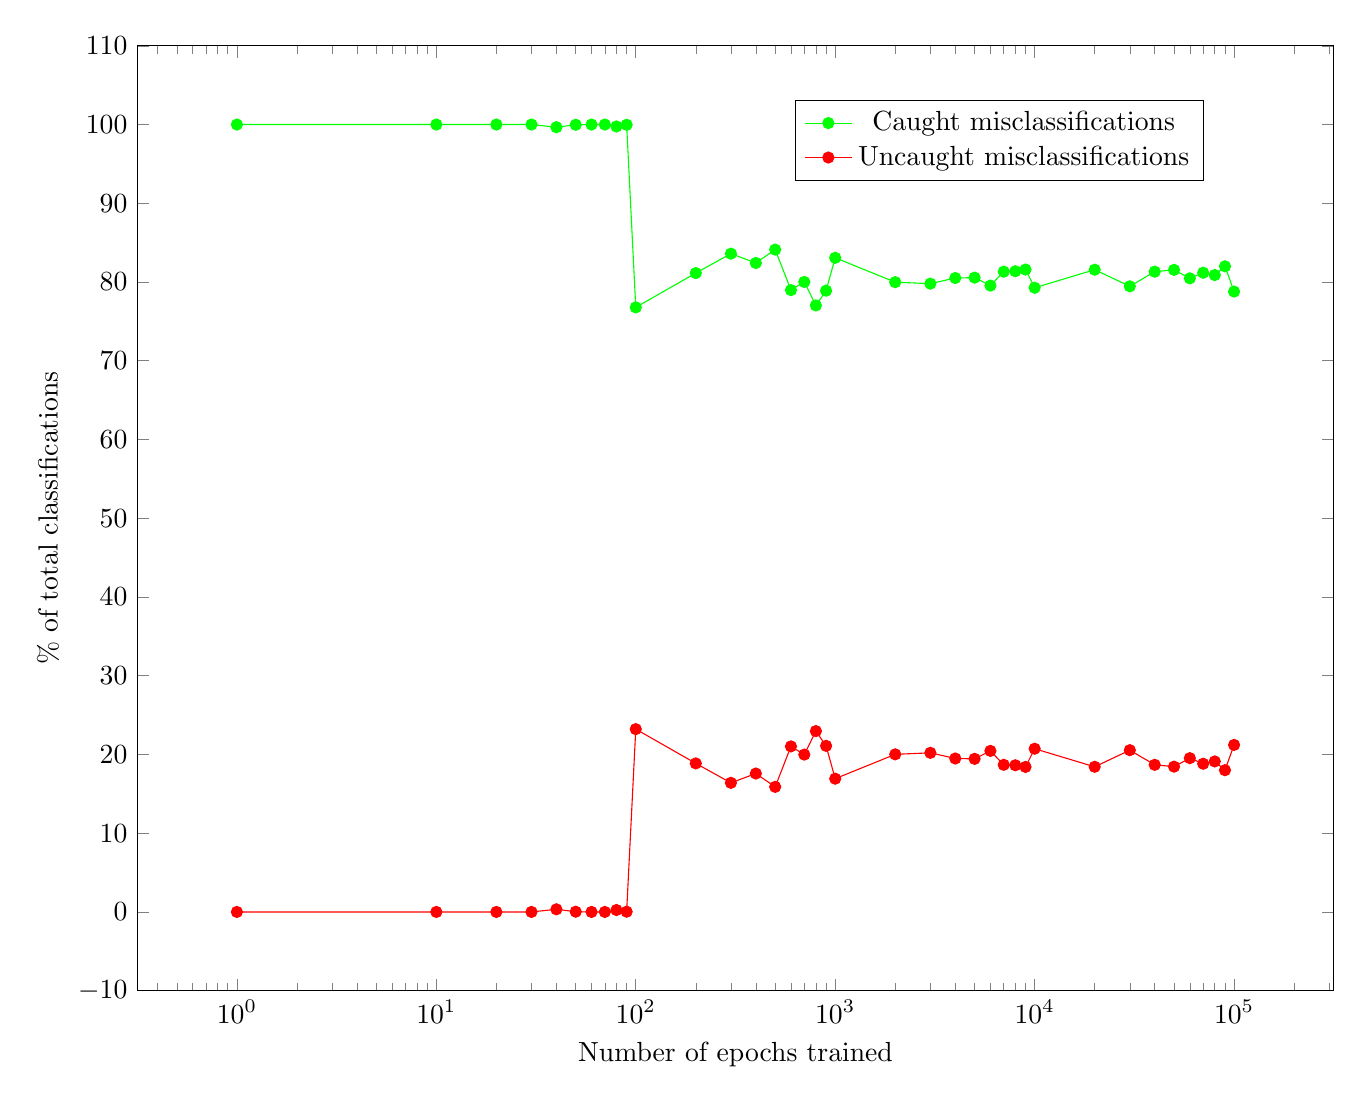
\begin{tikzpicture}
\begin{semilogxaxis}[
xlabel={Number of epochs trained},
ylabel={\% of total classifications},
x=1.1cm,
y=1.0mm, 
legend style={at={(0.55,0.9)},anchor=west}]

\addplot[color=green,mark=*] coordinates {	
	(1, 100.000000)
	(10, 100.000000)
	(20, 100.000000)
	(30, 100.000000)
	(40, 99.662552)
	(50, 99.968597)
	(60, 100.000000)
	(70, 100.000000)
	(80, 99.758133)
	(90, 99.968475)
	(100, 76.780945)
	(200, 81.134331)
	(300, 83.604851)
	(400, 82.419716)
	(500, 84.116234)
	(600, 78.973373)
	(700, 80.015221)
	(800, 77.028572)
	(900, 78.905663)
	(1000, 83.074722)
	(2000, 79.983315)
	(3000, 79.792389)
	(4000, 80.510559)
	(5000, 80.555107)
	(6000, 79.547066)
	(7000, 81.314125)
	(8000, 81.369659)
	(9000, 81.582603)
	(10000, 79.271027)
	(20000, 81.565376)
	(30000, 79.456421)
	(40000, 81.315414)
	(50000, 81.545204)
	(60000, 80.468216)
	(70000, 81.178162)
	(80000, 80.884285)
	(90000, 81.995102)
	(100000, 78.786835)
};

\addplot[color=red,mark=*] coordinates {
	(1, 0.000000)
	(10, 0.000000)
	(20, 0.000000)
	(30, 0.000000)
	(40, 0.337446)
	(50, 0.031402)
	(60, 0.000000)
	(70, 0.000000)
	(80, 0.241872)
	(90, 0.031525)
	(100, 23.219051)
	(200, 18.865665)
	(300, 16.395145)
	(400, 17.580284)
	(500, 15.883766)
	(600, 21.026627)
	(700, 19.984774)
	(800, 22.971428)
	(900, 21.094332)
	(1000, 16.925280)
	(2000, 20.016680)
	(3000, 20.207613)
	(4000, 19.489441)
	(5000, 19.444899)
	(6000, 20.452932)
	(7000, 18.685873)
	(8000, 18.630341)
	(9000, 18.417391)
	(10000, 20.728970)
	(20000, 18.434624)
	(30000, 20.543579)
	(40000, 18.684584)
	(50000, 18.454794)
	(60000, 19.531784)
	(70000, 18.821840)
	(80000, 19.115713)
	(90000, 18.004898)
	(100000, 21.213161)
};

\legend{Caught misclassifications, Uncaught misclassifications}
\end{semilogxaxis}%
\end{tikzpicture}%}
	\caption{Line graph showing the number of misclassifications made by the system with perturbed inputs \label{fig:sign-graphpert}}
\end{figure}

\begin{figure}[t]
	\centering
	\scalebox{1}{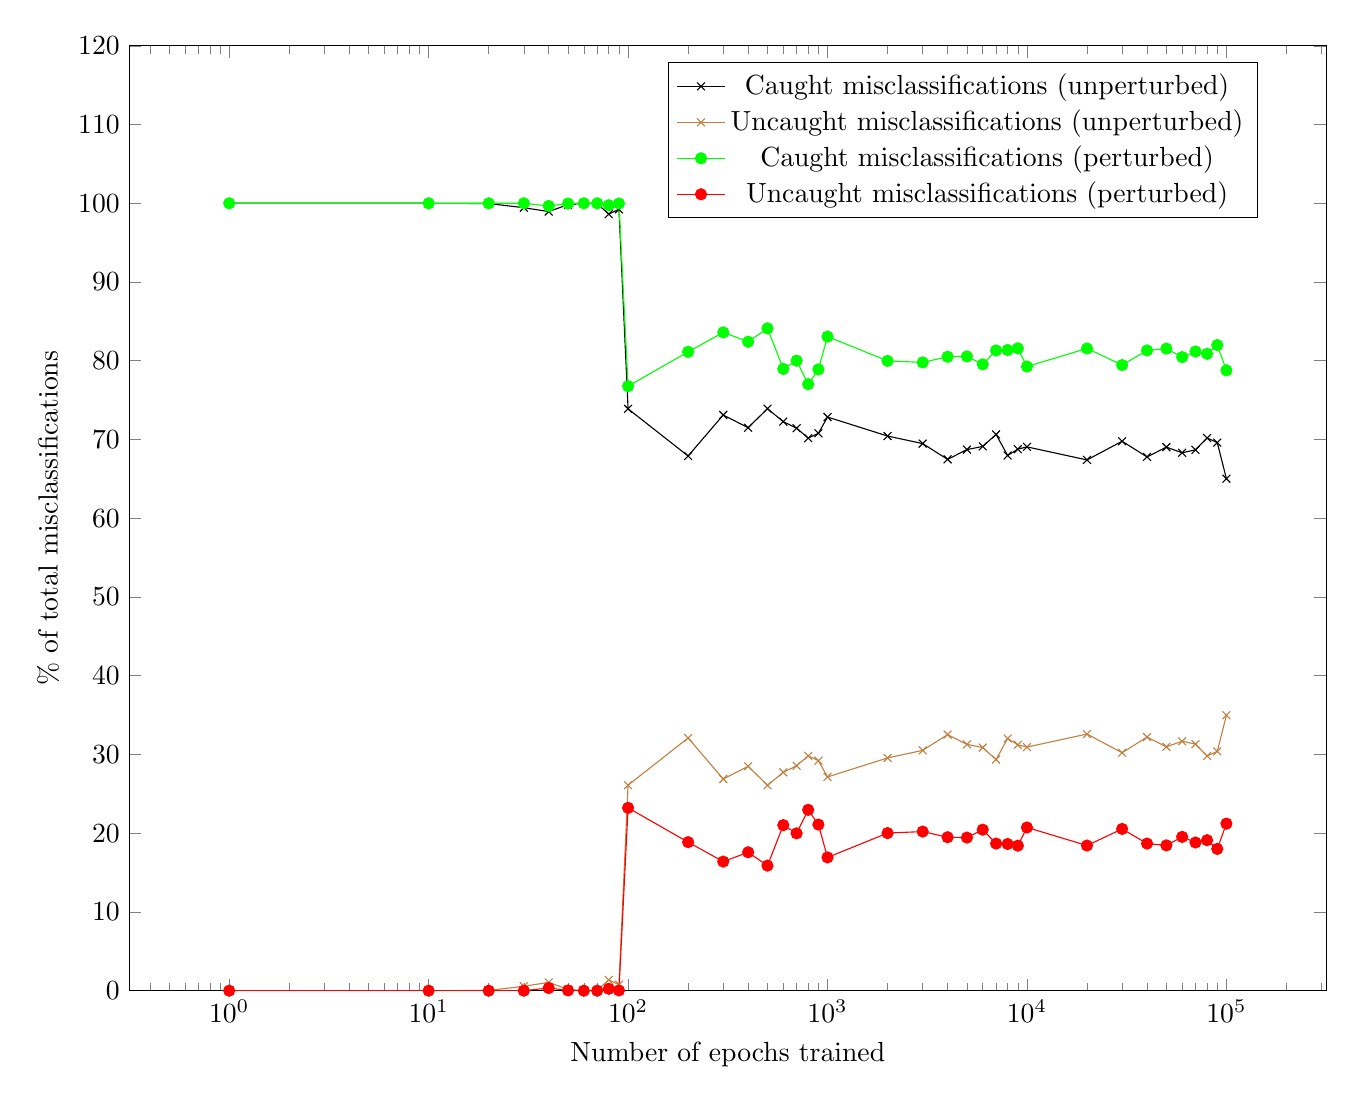
\begin{tikzpicture}
\begin{semilogxaxis}[
xlabel={Number of epochs trained},
ylabel={\% of total misclassifications},
x=1.1cm, y=1.0mm, 
ymin=0, ymax=120,
legend style={at={(0.45,0.9)},anchor=west}]

\addplot[color=black,mark=x] coordinates {
	(1, 100.000000)
	(10, 100.000000)
	(20, 99.968513)
	(30, 99.438622)
	(40, 98.948822)
	(50, 99.831619)
	(60, 100.000000)
	(70, 99.946243)
	(80, 98.629845)
	(90, 99.235352)
	(100, 73.896217)
	(200, 67.904327)
	(300, 73.114166)
	(400, 71.500191)
	(500, 73.917786)
	(600, 72.264412)
	(700, 71.438644)
	(800, 70.175438)
	(900, 70.787399)
	(1000, 72.854225)
	(2000, 70.439842)
	(3000, 69.480080)
	(4000, 67.477409)
	(5000, 68.717560)
	(6000, 69.121811)
	(7000, 70.645164)
	(8000, 67.972473)
	(9000, 68.772896)
	(10000, 69.063011)
	(20000, 67.405907)
	(30000, 69.780220)
	(40000, 67.787842)
	(50000, 69.032257)
	(60000, 68.315018)
	(70000, 68.693977)
	(80000, 70.194382)
	(90000, 69.604439)
	(100000, 65.025040)
};

\addplot[color=brown,mark=x] coordinates {	
	(1, 0.000000)
	(10, 0.000000)
	(20, 0.031486)
	(30, 0.561380)
	(40, 1.051184)
	(50, 0.168381)
	(60, 0.000000)
	(70, 0.053759)
	(80, 1.370155)
	(90, 0.764649)
	(100, 26.103786)
	(200, 32.095673)
	(300, 26.885832)
	(400, 28.499805)
	(500, 26.082212)
	(600, 27.735594)
	(700, 28.561354)
	(800, 29.824560)
	(900, 29.212601)
	(1000, 27.145777)
	(2000, 29.560154)
	(3000, 30.519920)
	(4000, 32.522587)
	(5000, 31.282434)
	(6000, 30.878185)
	(7000, 29.354836)
	(8000, 32.027523)
	(9000, 31.227106)
	(10000, 30.936995)
	(20000, 32.594090)
	(30000, 30.219782)
	(40000, 32.212166)
	(50000, 30.967743)
	(60000, 31.684982)
	(70000, 31.306025)
	(80000, 29.805618)
	(90000, 30.395559)
	(100000, 34.974957)
};

\addplot[color=green,mark=*] coordinates {	
	(1, 100.000000)
	(10, 100.000000)
	(20, 100.000000)
	(30, 100.000000)
	(40, 99.662552)
	(50, 99.968597)
	(60, 100.000000)
	(70, 100.000000)
	(80, 99.758133)
	(90, 99.968475)
	(100, 76.780945)
	(200, 81.134331)
	(300, 83.604851)
	(400, 82.419716)
	(500, 84.116234)
	(600, 78.973373)
	(700, 80.015221)
	(800, 77.028572)
	(900, 78.905663)
	(1000, 83.074722)
	(2000, 79.983315)
	(3000, 79.792389)
	(4000, 80.510559)
	(5000, 80.555107)
	(6000, 79.547066)
	(7000, 81.314125)
	(8000, 81.369659)
	(9000, 81.582603)
	(10000, 79.271027)
	(20000, 81.565376)
	(30000, 79.456421)
	(40000, 81.315414)
	(50000, 81.545204)
	(60000, 80.468216)
	(70000, 81.178162)
	(80000, 80.884285)
	(90000, 81.995102)
	(100000, 78.786835)
};

\addplot[color=red,mark=*] coordinates {
	(1, 0.000000)
	(10, 0.000000)
	(20, 0.000000)
	(30, 0.000000)
	(40, 0.337446)
	(50, 0.031402)
	(60, 0.000000)
	(70, 0.000000)
	(80, 0.241872)
	(90, 0.031525)
	(100, 23.219051)
	(200, 18.865665)
	(300, 16.395145)
	(400, 17.580284)
	(500, 15.883766)
	(600, 21.026627)
	(700, 19.984774)
	(800, 22.971428)
	(900, 21.094332)
	(1000, 16.925280)
	(2000, 20.016680)
	(3000, 20.207613)
	(4000, 19.489441)
	(5000, 19.444899)
	(6000, 20.452932)
	(7000, 18.685873)
	(8000, 18.630341)
	(9000, 18.417391)
	(10000, 20.728970)
	(20000, 18.434624)
	(30000, 20.543579)
	(40000, 18.684584)
	(50000, 18.454794)
	(60000, 19.531784)
	(70000, 18.821840)
	(80000, 19.115713)
	(90000, 18.004898)
	(100000, 21.213161)
};

\legend{Caught misclassifications (unperturbed), Uncaught misclassifications (unperturbed), Caught misclassifications (perturbed), Uncaught misclassifications (perturbed)}
\end{semilogxaxis}%
\end{tikzpicture}%}
	\caption{Line graph showing the number of misclassifications made by the system with all inputs \label{fig:sign-graphboth}}
\end{figure}

%\todo{Add table showing how \ac{MNN} affects the prediction accuracy}

\subsection{An \ac{AV} System Using \acf{MNN2C}}
\ac{MNN2C}, introduced in Section~\ref{sec:mnn2c}, creates time-predictable, modular \acfp{MNN} for C from existing Keras (with Tensorflow) trained \acp{ANN}. 
This compiler makes implementing \acfp{SNN} in C easy and safe.
For the purposes of testing and demonstration, the complex \ac{MNN} used in this chapter, shown in Figure~\ref{fig:mnn}, was trained in Python, using Keras and the exact same images used to train the original system.
This \ac{MNN} was then described in the \ac{MNN2C} format, and modular C code was generated to initialise, run and incorporate the \ac{MNN}.
To show the efficacy of \ac{MNN2C}, the generated \ac{MNN} was implemented in an identical system to the original, and run with the same tests. 
It has already been shown that \ac{MNN2C} generates outputs identical to the Keras trained \acp{ANN} with a one hundred-thousandth tolerance, so the output of each individual \ac{ANN} is not being tested, rather that the system as a whole runs as the original does.
Additionally, the time-predictable \ac{MNN} was run through the Patmos \ac{WCET} tool in order to get the \ac{WCET} and \ac{WCRT} of the \ac{MNN}.

\subsubsection{Results of an \ac{MNN2C} Generated \ac{AV} System}
\begin{table}[h]
	\centering
	\resizebox{\textwidth}{!}{%
		\begin{tabular}{|p{0.17\linewidth}||p{0.17\linewidth}|p{0.17\linewidth}|p{0.17\linewidth}|p{0.17\linewidth}|}
			\hline
			Object classified & No. of misclassifications (\%) & Caught misclassifications (\%) & False negatives (\%) & Uncaught misclassifications (\%) \\ \hline
			Person & 0.37 & 0.35 & 3.89 & 3.92 \\ \hline
			Vehicle & 8.67 & 8.53 & 1.62 & 1.76 \\ \hline
			Sign & 7.58 & 7.07 & 11.94 & 12.44 \\ \hline
			Nothing & 8.39 & 8.27 & 0.05 & 0.16 \\ \hline
			All & 25.01 & 24.22 & 17.50 & 18.29 \\ \hline
		\end{tabular}%
	}
	\caption{Table showing the best results of the \ac{AV} prediction \ac{MNN} using original images, generated by \ac{MNN2C} and trained for 100 epochs}
	\label{tbl:sign-resmnn}
\end{table}

\begin{table}[h]
	\centering
	\resizebox{\textwidth}{!}{%
		\begin{tabular}{|p{0.17\linewidth}||p{0.17\linewidth}|p{0.17\linewidth}|p{0.17\linewidth}|p{0.17\linewidth}|}
			\hline
			Object classified & No. of misclassifications (\%) & Caught misclassifications (\%) & False negatives (\%) & Uncaught misclassifications (\%) \\ \hline
			Person & 0.23 & 0.23 & 5.26 & 5.26 \\ \hline
			Vehicle & 9.52 & 9.32 & 2.04 & 2.25 \\ \hline
			Sign & 23.75 & 21.69 & 14.14 & 16.20 \\ \hline
			Nothing & 8.44 & 8.37 & 0.00 & 0.07 \\ \hline
			All & 41.95 & 39.61 & 21.44 & 23.78 \\ \hline
		\end{tabular}%
	}
	\caption{Table showing the best results of the \ac{AV} prediction \ac{MNN} using perturbed images, generated by \ac{MNN2C} and trained for 100 epochs}
	\label{tbl:sign-resmnnpert}
\end{table}



















